\section{系统运行}

\subsection{用户模块}

登陆模块包括用户的注册、登陆、找回密码、邮箱验证等功能,登陆界面的记住我可以设置浏览器中的cookie的过期时间为7天,登陆如图5.1所示,注册如图5.2所示,找回密码如图5.3所示,个人中心如图5.4所示。

\begin{figure}[thbp!]
	\centering
	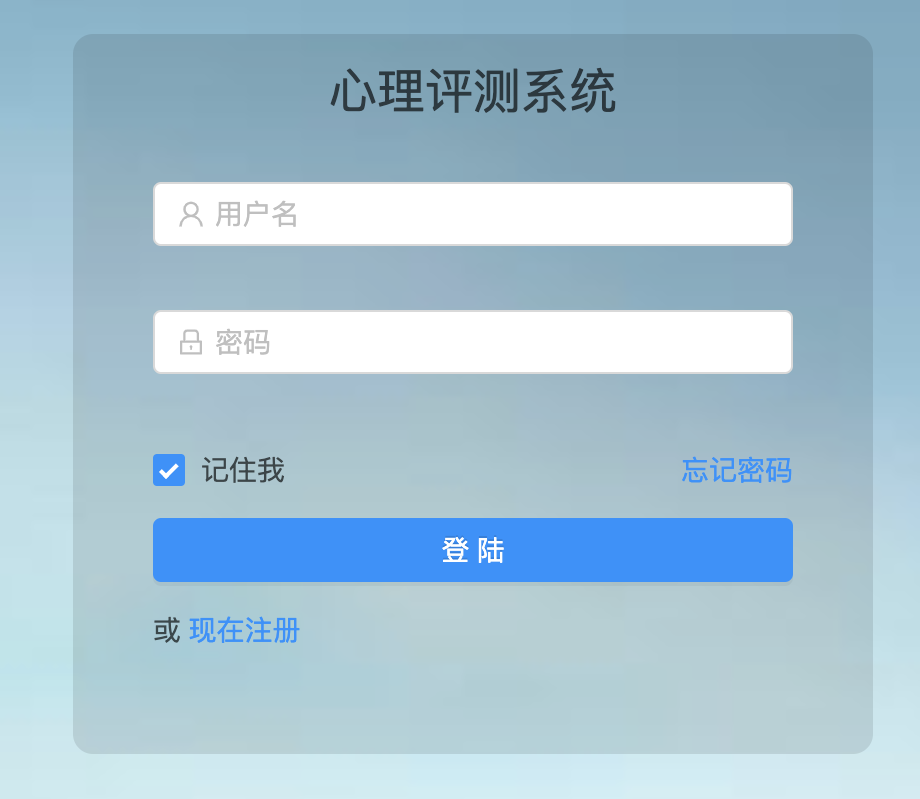
\includegraphics[width=0.6\linewidth]{figure/login}
	\label{fig:login} \\
	图5.1 登陆界面
\end{figure}

\begin{figure}[thbp!]
	\centering
	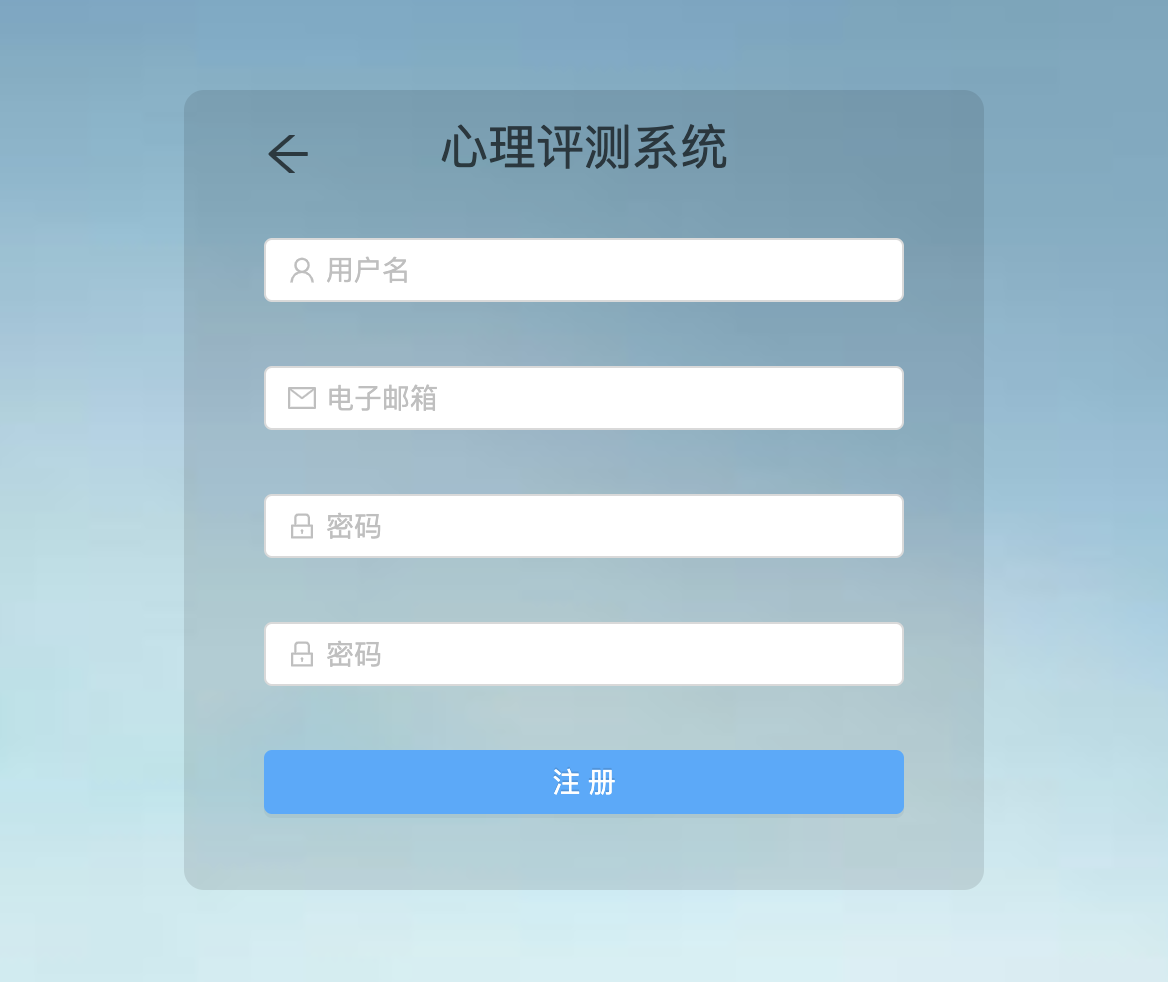
\includegraphics[width=0.5\linewidth]{figure/register}
	\label{fig:register} \\
	图5.2 注册界面
\end{figure}

\begin{figure}[thbp!]
	\centering
	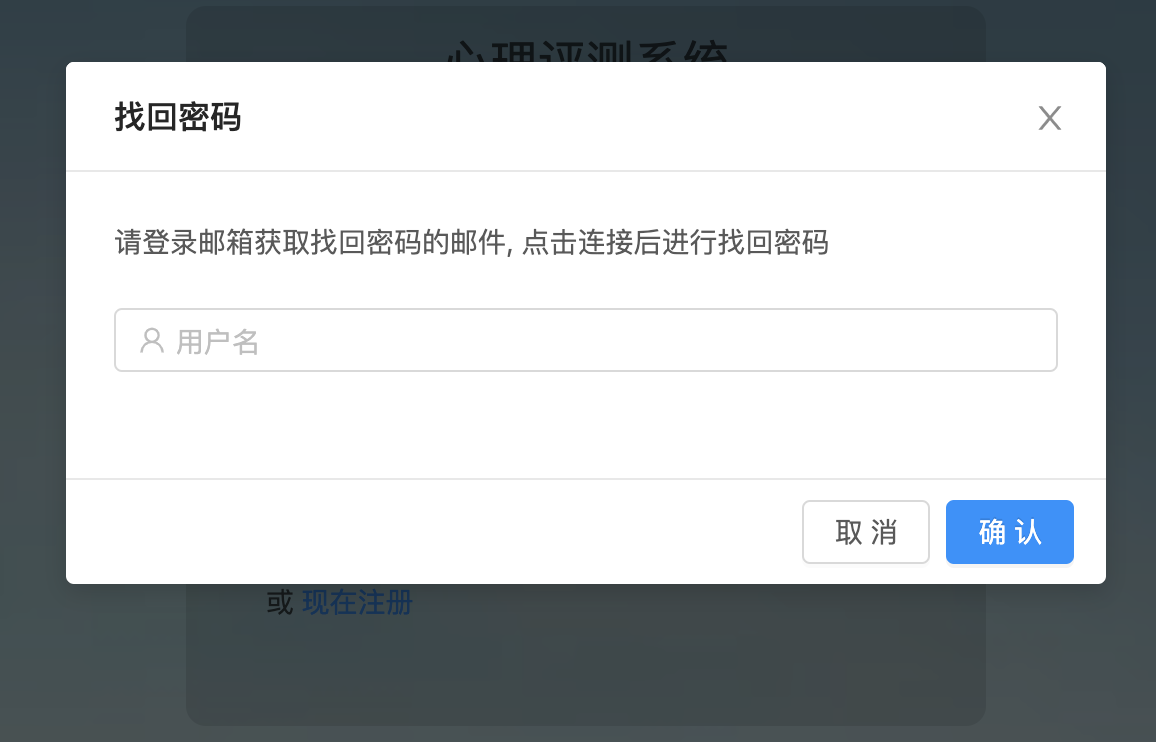
\includegraphics[height=0.35\linewidth]{figure/find_password}
	\label{fig:find_password} \\
	图5.3 找回密码
\end{figure}

\begin{figure}[thbp!]
	\centering
	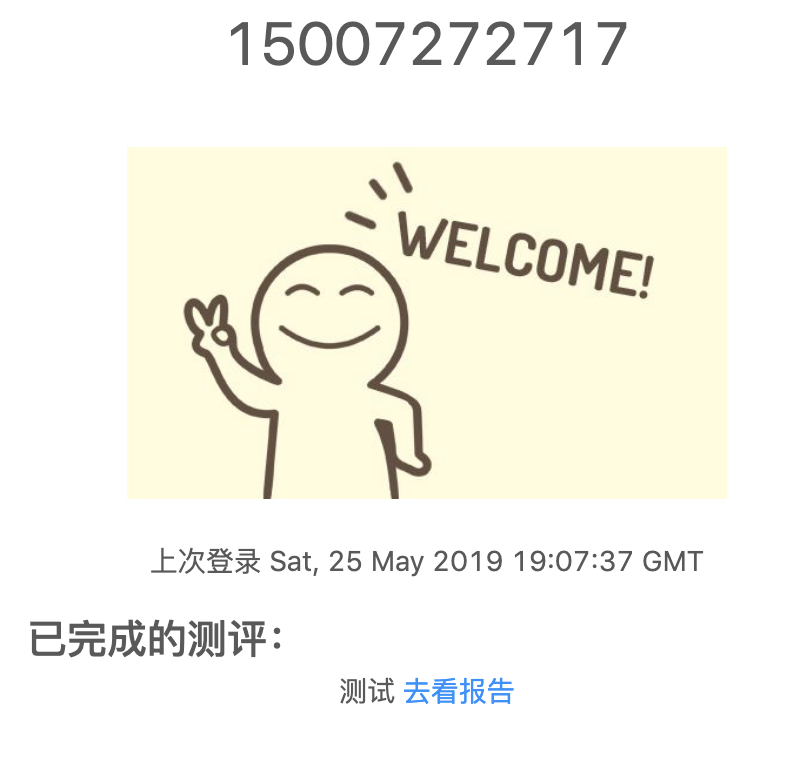
\includegraphics[height=0.35\linewidth]{figure/main}
	\label{fig:main} \\
	图5.4 个人中心
\end{figure}

\subsection{管理中心}

管理中心是管理员对试卷、用户、成绩进行筛选的模块,管理试卷如图5.5所示,管理用户如图5.6所示,可以更改用户的权限、删除用户、上传文件批量增加用户,筛选成绩如图5.7所示。

\begin{figure}[thbp!]
	\centering
	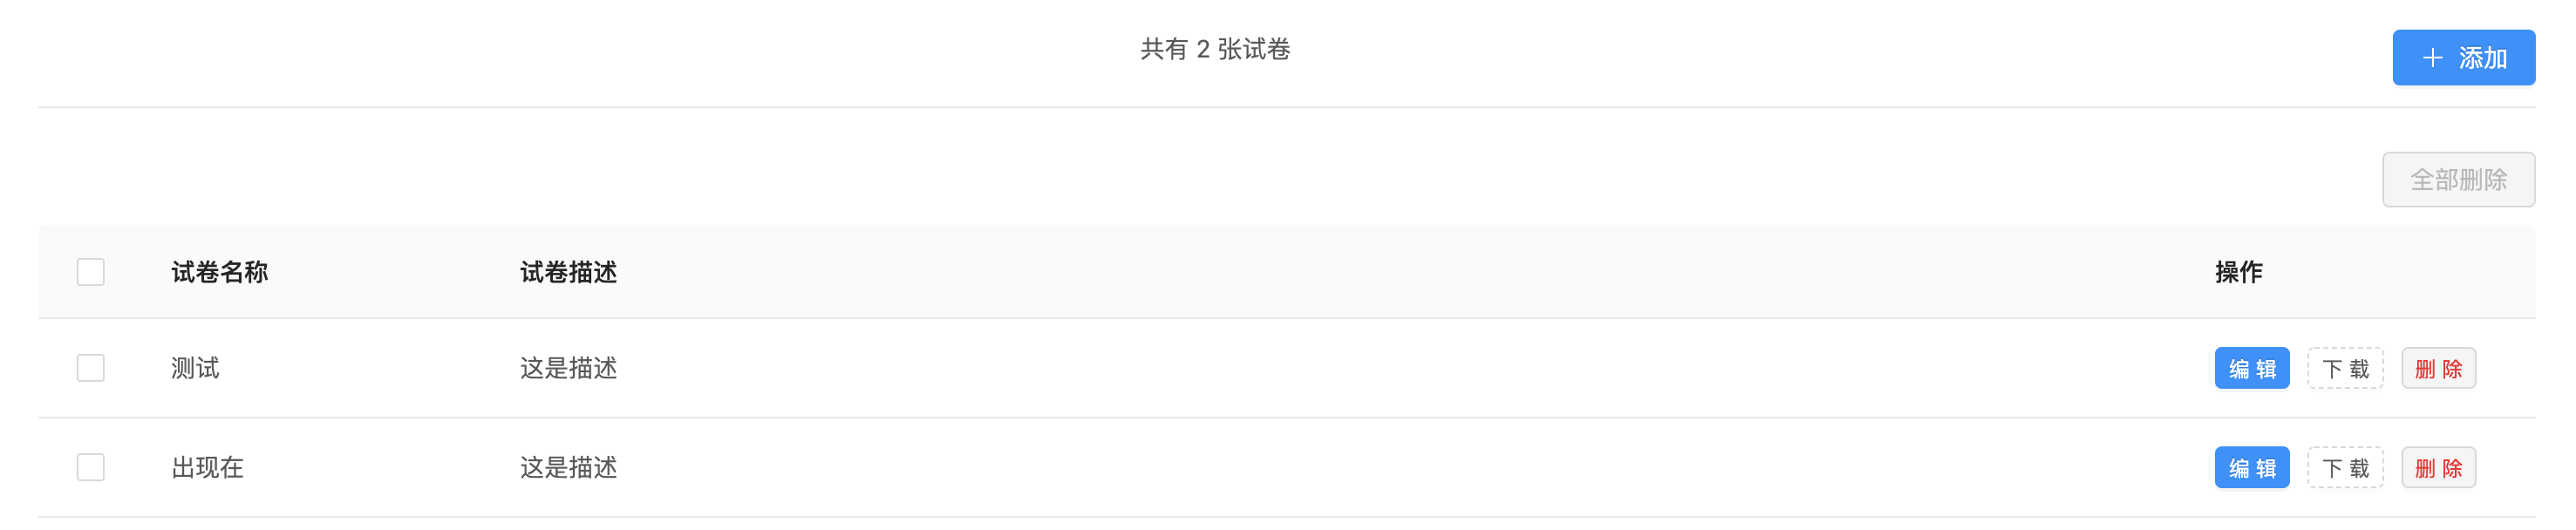
\includegraphics[width=1.0\linewidth]{figure/admin_paper}
	\label{fig:admin_paper} \\
	图5.5 管理试卷
\end{figure}

\begin{figure}[thbp!]
	\centering
	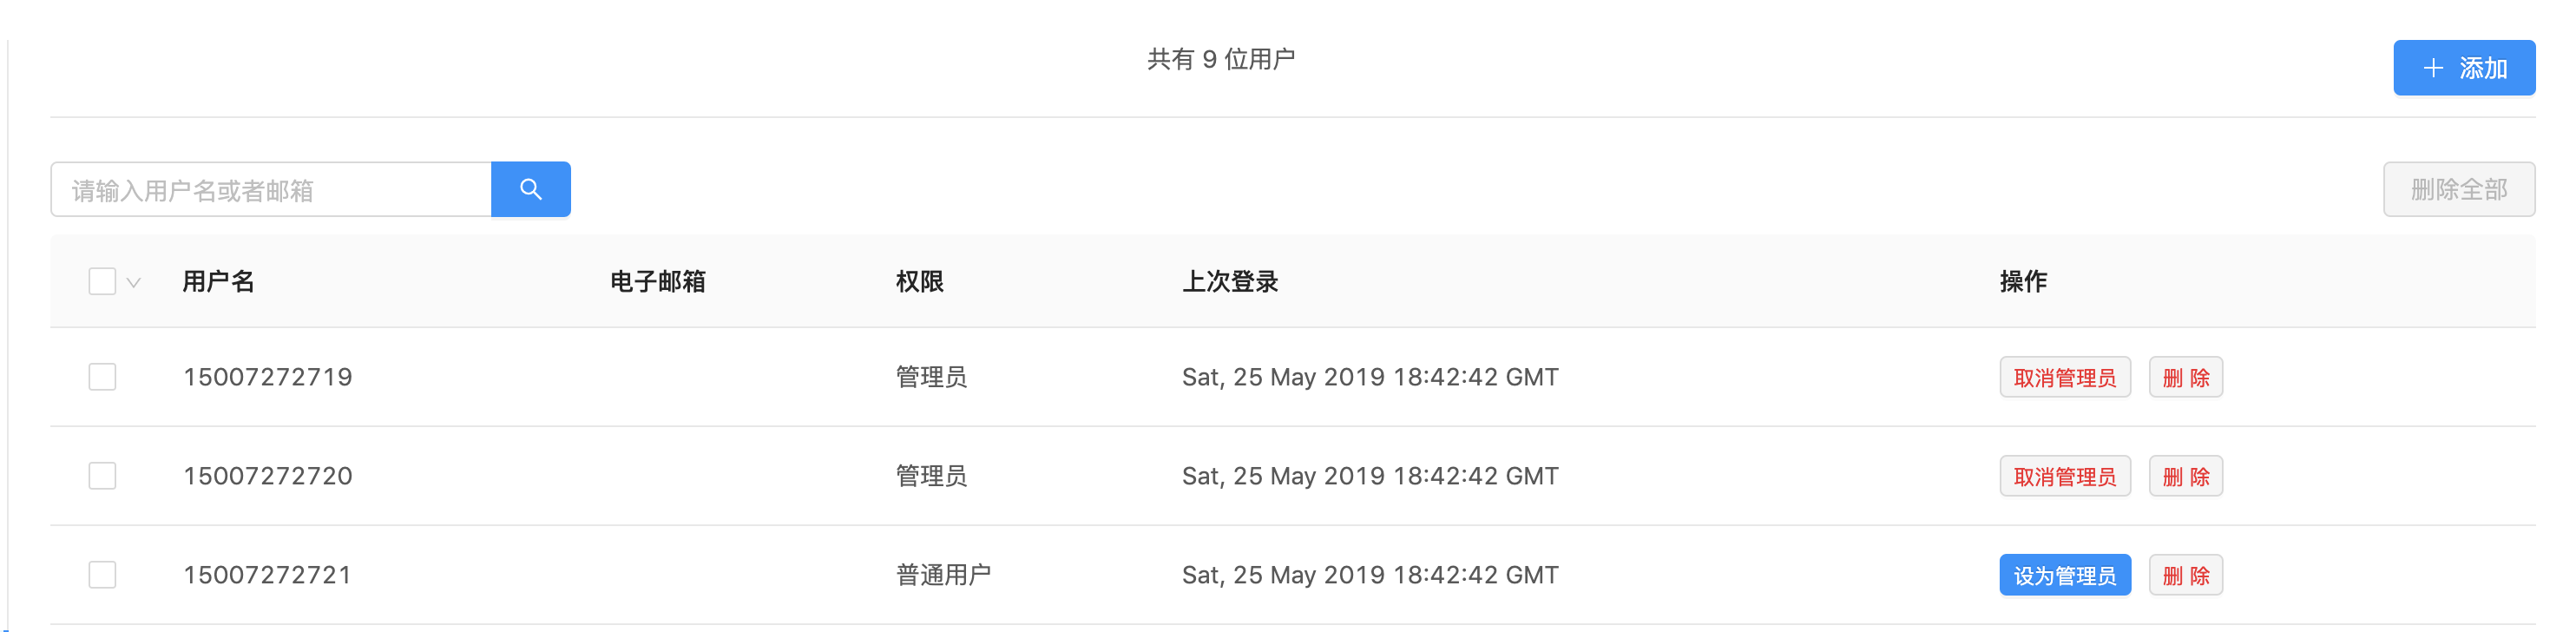
\includegraphics[width=1.0\linewidth]{figure/admin_user}
	\label{fig:admin_user} \\
	图5.6 管理用户
\end{figure}

\begin{figure}[thbp!]
	\centering
	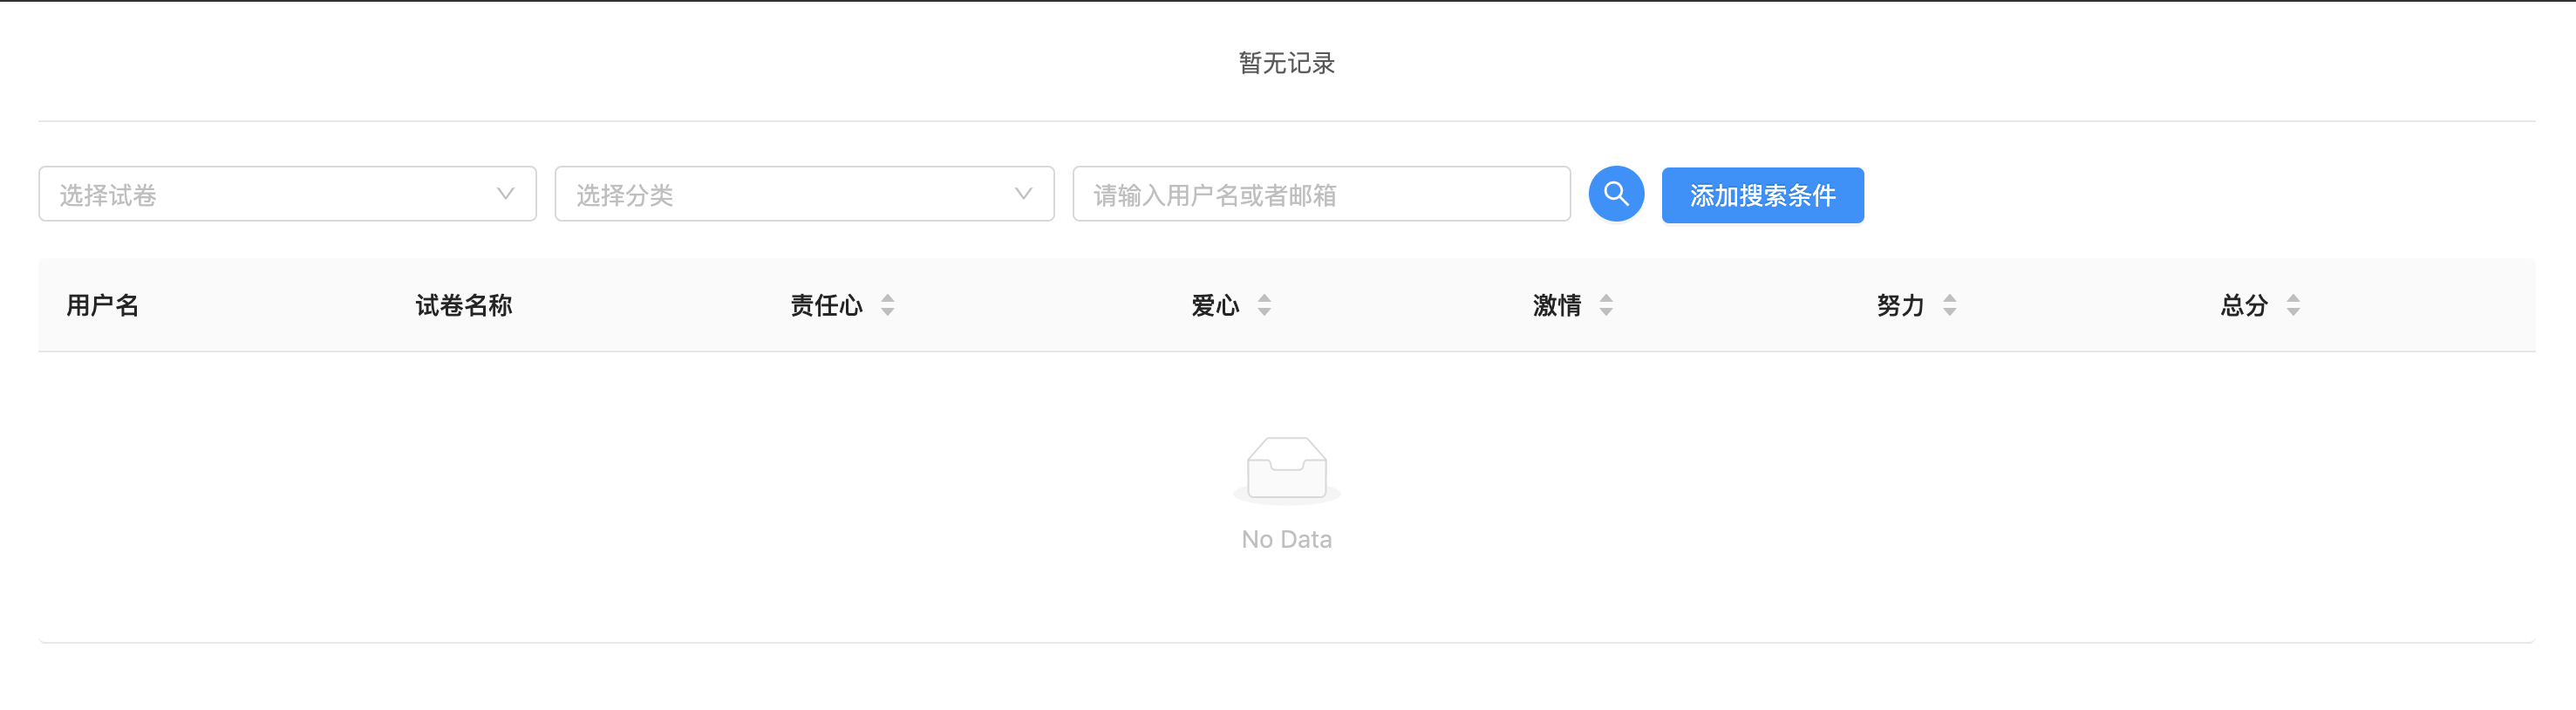
\includegraphics[width=1.0\linewidth]{figure/admin_grade}
	\label{fig:admin_grade} \\
	图5.7 筛选成绩
\end{figure}

\subsection{评测中心}

评测中心是用户参加评测和查看报告的模块,具体评测如图5.9所示,评测的结果如图5.10所示,可以看到用户自己的各个指标的得分、试卷的平均分、自己的分数高于做试卷的人数的比例、自己试卷的评论和最多人选的答案。

\begin{figure}[thbp!]
	\centering
	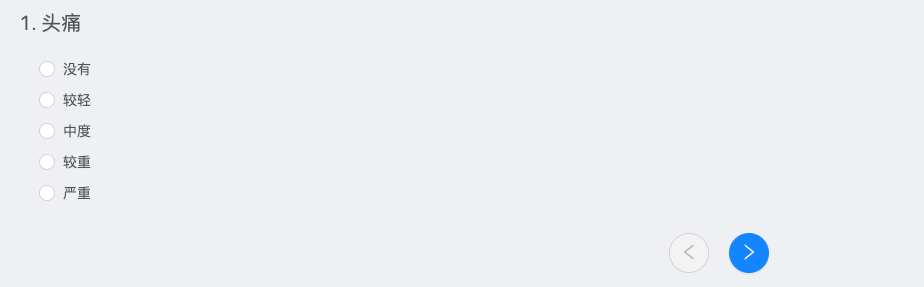
\includegraphics[width=0.7\linewidth]{figure/test_main}
	\label{fig:test_main} \\
	图5.8 评测内容
\end{figure}

\begin{figure}[thbp!]
	\centering
	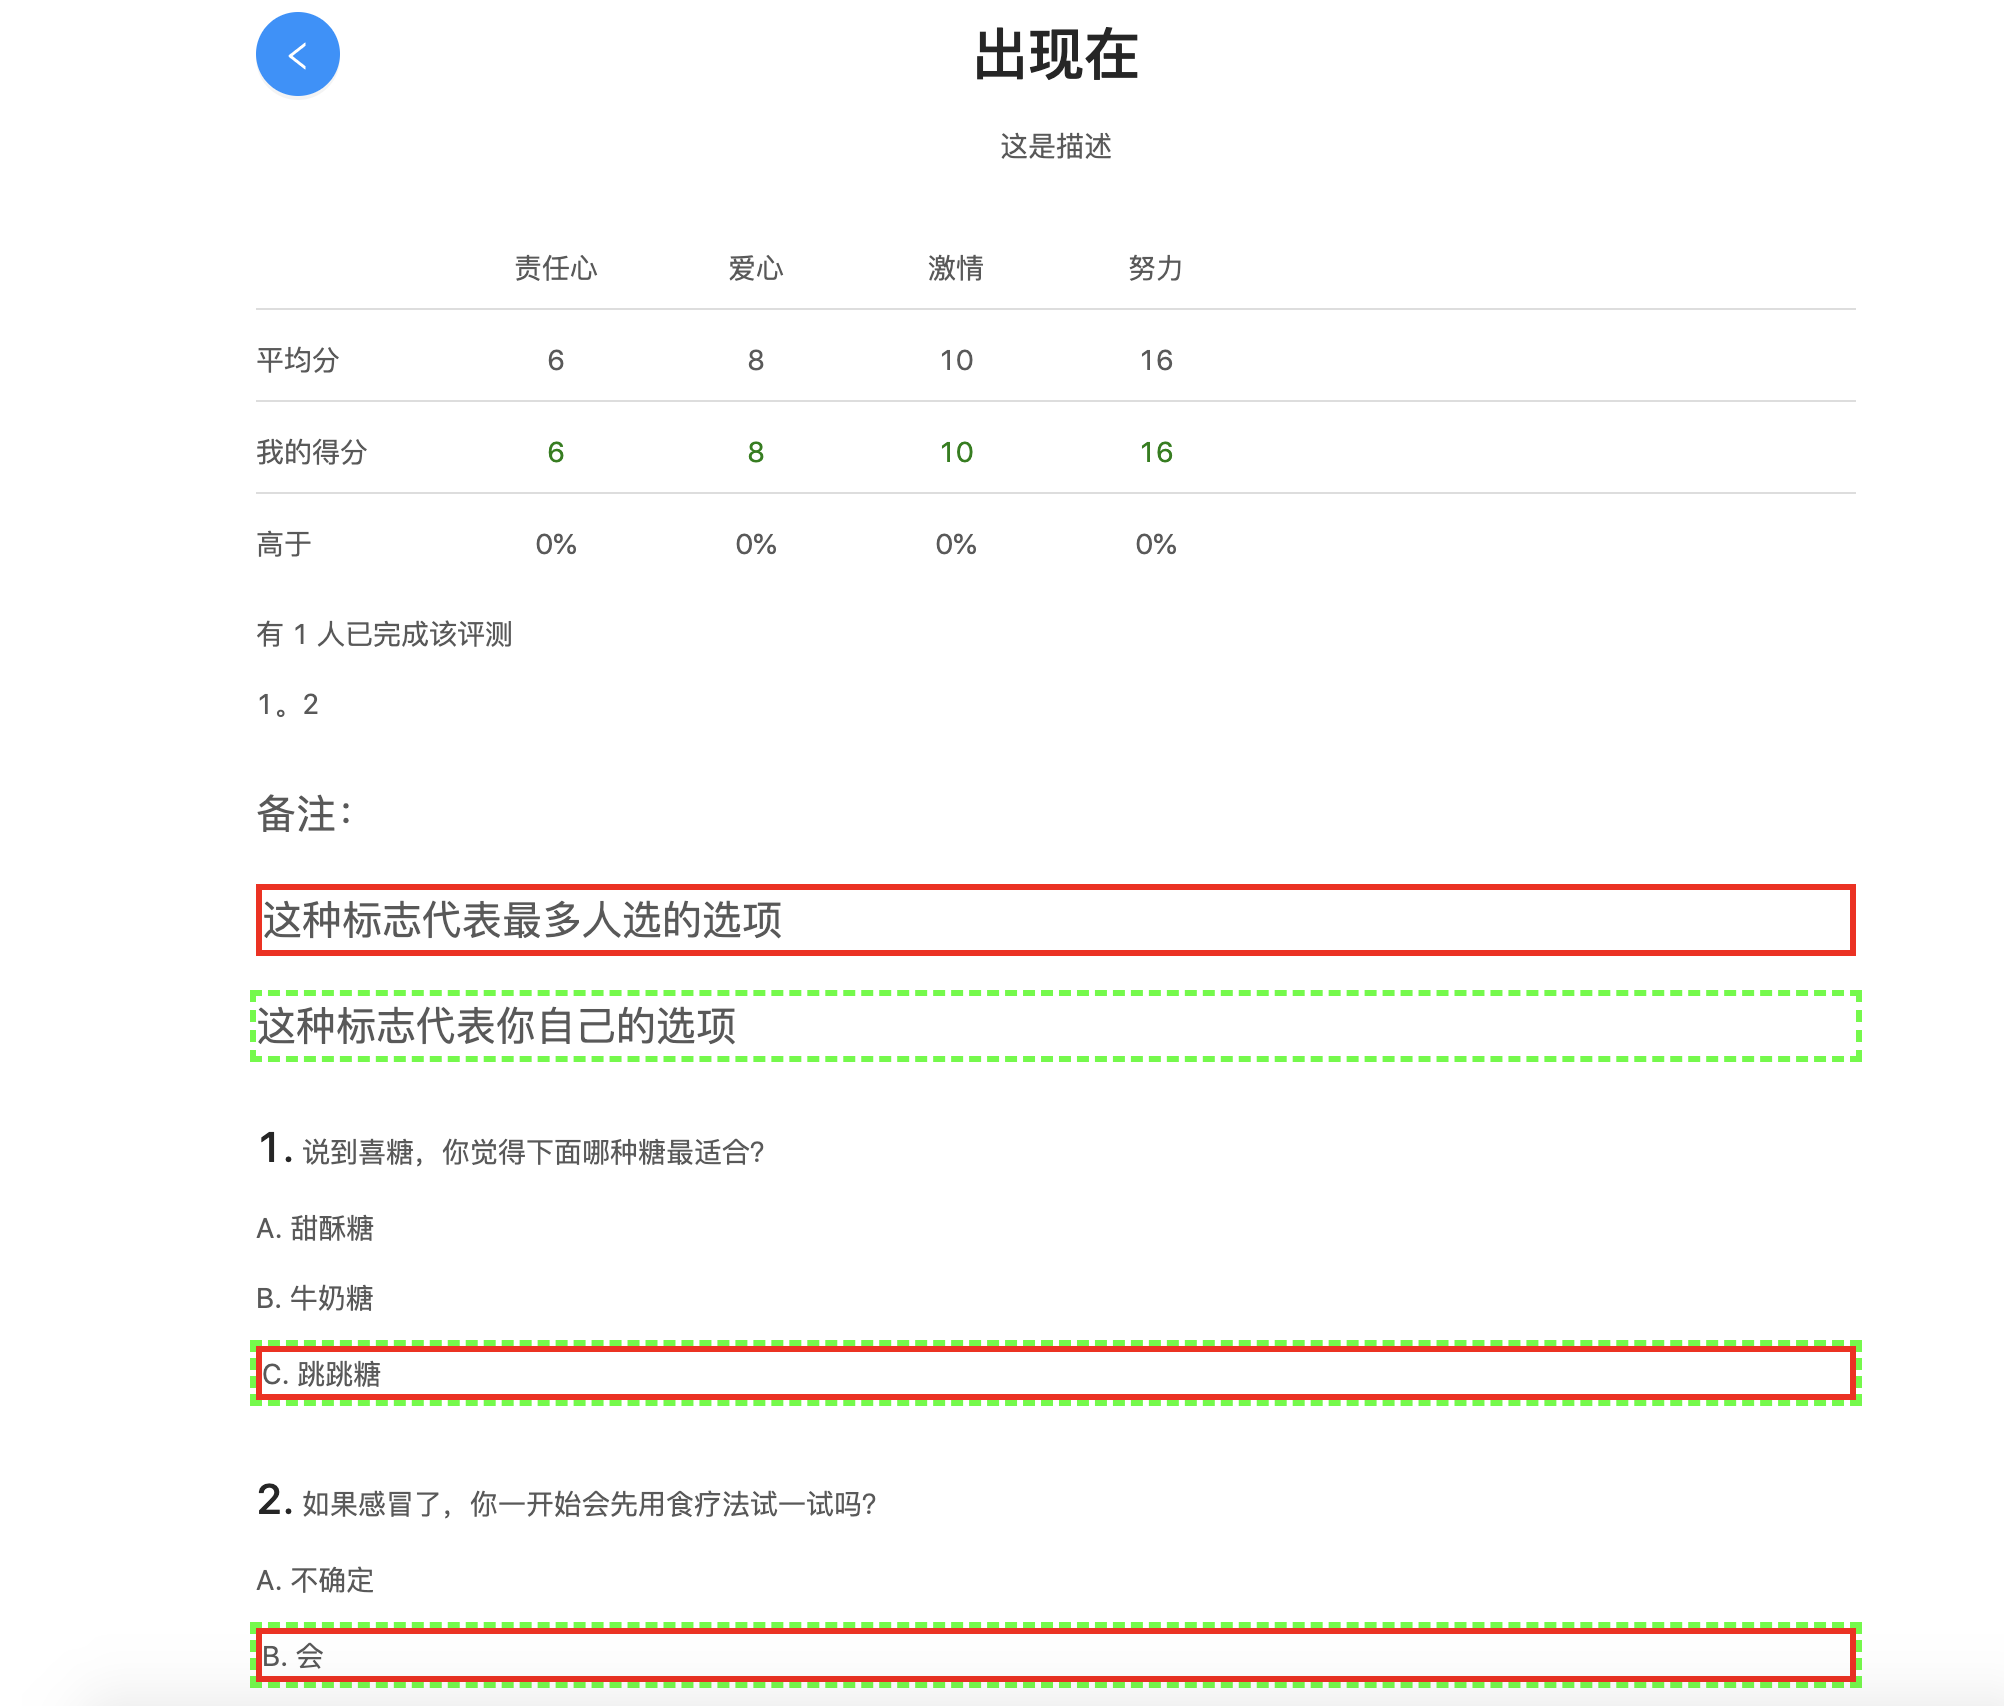
\includegraphics[height=0.7\linewidth]{figure/result_main}
	\label{fig:result_main} \\
	图5.9 评测结果
\end{figure}

